\documentclass[12pt]{report}

\usepackage{amssymb,amsthm}
\usepackage{amsmath,color}
%\usepackage{dsfont}
\usepackage{setspace}
\usepackage{graphicx}
\usepackage{multicol}
\usepackage[document]{ragged2e}

\usepackage{fancyhdr}
% \usepackage[]{classicthesis}

\def\changemargin#1#2{\list{}{\rightmargin#2\leftmargin#1}\item[]}
\let\endchangemargin=\endlist 

\def\w{\mathtt w}
\def\K{\mathcal K}
\def\N{\mathbb N}
\def\R{\mathcal R}
\def\l{\ell}
\def\S{\mathcal S}
\def\Z{\mathbb Z}
\def\ora{\overrightarrow}


\newtheorem{theorem}{Theorem}[section]
\newtheorem{corollary}{Corollary}[theorem]
\newtheorem{lemma}[theorem]{Lemma}


\begin{document}

\begin{center}
\LARGE{\textbf{Indian Institute of Technology, Delhi}}\\
\vspace{0.8cm}
\large{\textbf{Design Practices in Computer Science}}\\[5pt]
\large{\textbf{COP290}}\\[5pt]
% \large{\textbf{Mathematical Model}}\\[5pt]
%by \\
\vspace{0.5cm}

\large{\textbf{Starling Simulation }}
% \large{\textbf{\\to understand the Flocking behaviour of birds}}\\[5pt]


%\vspace{1in}

\begin{center}

\includegraphics[height=5cm]{iitd.eps}
\end{center}
\vspace{0.2cm}

\textbf{April 18, 2018} \\
\textbf{Department of Computer Science and Engineering} \\
\textbf{Indian Institute of Technology, Delhi}\\


\vspace{1.5cm}


\begin{multicols*}{2}

\begin{flushleft}

\textit{Authors :\\ }


\textbf{Udit Jain} \\
(2016CS10327)\\
\textbf{Shashank Goel}
(2016CS10332)\\

\end{flushleft}


\columnbreak

\begin{flushleft}

\textit{\\Supervisor :\\ }
\textbf{Prof. Subhashish Bannerjee} \\[5pt]

\end{flushleft}

\end{multicols*}

\end{center}

\newpage



\begin{center}
\Large \bf ABSTRACT
\end{center}
\vspace{0.2in}

We are going to design and implement a Starling Simulation that will help us understand the Flocking behaviour of birds. Computer Science term for this simulation is Boids.
\\
\vspace{0.3cm}
The simulation software will have the following functionalities:

\begin{enumerate}
  \item
  We will be able to interactively input or read from a file :
  \begin{itemize}
    \item
    Degree of Seperation, Cohesion, Alignment.  
    \item
    Speed of boids .
  \end{itemize}
  \item
  We can interactively add / remove \textit{ boids and obstacles } based on combination of inputs from keyboard and mouse. 
  \item
  Get the color of boids based by grouping on speed, flock, direction .
  \item
  Calcuate and display average Velocity and Accleration vector of boid groups and global flock dynamically.
  \item
  Calcuate and display average Kinetic Energy of boid groups and global flock dynamically.
\end{enumerate}


\vspace{0.5cm}
Future scope of the problem may include:

\begin{enumerate}
  \item
  Interactively control the Gravity vector and see it's effect on the flock .
  \item
  Adding and measuring the effect of Wind speed / direction and Drag on the flock .
\end{enumerate}


\vspace{0.5cm}


In this design project, we shall work as observers, developers and algorithm enthusiasts to understand the ways and finding different means to approach and tackle the objectives in a more well defined mathematical way. 

\vspace{0.2cm}
We shall work with full confidence and zeal to achieve the goal or reach to quite an end of the problem so that using our lemmas, proofs and knowledge, someday a perfect model can be implemented using a software by some other Computer Explorer. As a matter of interest, we just wish to argue that these things can be computed by our brain so we do hope to find a solution to this problem using machine learning algorithms. Since, Machine Learning algorithms are more or less based on Mathematical matrices, with the use of computer graphics, we expect to find a start with matrices that we have dealt with further in this report. 

\newpage

\tableofcontents

\newpage

% \setcounter{secnumdepth}{-1} % to unNumber introduction

\chapter{Introduction}

Boids is an artificial life program, developed by Craig Reynolds in 1986,
which simulates the flocking behaviour of birds. His paper on this topic
was published in 1987 in the proceedings of the ACM SIGGRAPH con-
ference. The name ”boid” corresponds to a shortened version of ”bird-oid
object”, which refers to a bird-like object.

\vspace{1cm}

As with most artificial life simulations, Boids is an example of emergent
behavior; that is, the complexity of Boids arises from the interaction of in-
dividual agents (the boids, in this case) adhering to a set of simple rules.
The rules applied in the simplest Boids world are as follows:

\begin{itemize}
  \item
  \textbf{\textit{Seperation}} : Steer to avoid crowding of local flockmates
    \begin{center}
      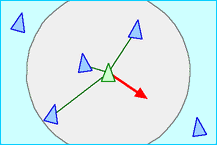
\includegraphics[height=5cm]{Rule_separation.png}
    \end{center}
  \item
  \textbf{\textit{Alignment}} : Steer towards the average heading of local flockmates.
  \begin{center}
    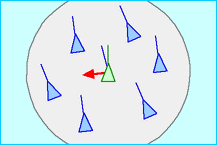
\includegraphics[height=5cm]{Rule_alignment.png}
  \end{center}
  \item
  \textbf{\textit{Cohesion}} : Steer to move toward the average position (Center of Mass) of local flockmates.
    \begin{center}
    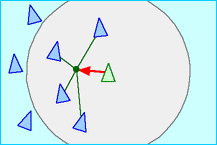
\includegraphics[height=5cm]{Rule_cohesion.png}
  \end{center}
\end{itemize}

\vspace{0.5cm}
More complex rules can be added, such as obstacle avoidance and goal seeking .\\

\vspace{0.5cm}

The following objectives are aimed to be discussed in this paper:
\begin{itemize}
  \item
  Defining the problem.
  % Support you design decisions ? 
  \item
  Discussing how a simulation is modeled, what are the diffrent padigrams.
  % logical time (when equal to) real time, for loop(not giving perefrence to one starlilng) concurrency (Showing it is equal because all threads have to access each other's memory, locking problem ?) ? repeated ? ||| Bound on number of starlings ? Experimenation with hyperparameters ?
  % Changing according to some hyper-parameters ? 

  \item
  What set of rules govern bird in flocks.
  % Power, drag, float force, Can birds sustain that ? Do we limit 
  \item
  What model is to be adopted for interplay of starlings with the environment.
  \item
  What parameters can be varied to see interesting patterns.
  % (dynamic and average) power, KE . Energy expenditure, food ? , 
  \item
  Intresting Obeservations on varying diffrent parameters in simulation.
\end{itemize}

\chapter{Defining the problem}
\secion{Introduction}
\subsection{Why do we care about bird flocking patterns ?}
\secion{How do we study them ?}

\chapter{Modelling a Simulation}
\secion{Introduction}
\subsection{What's a simulation ?}
\secion{Types of Simulation}
\subsection{Key Aspects}


\chapter{Conclusion}


% \begin{thebibliography}{9}


% \bibitem{ALM}
% P. Allen, B. Landman and H. Meeks, New Bounds on van der Waerden type numbers for Generalized $3$-term Arithmetic Progressions, {\it arXiv: 1201.3842v2}


% \bibitem{BL}
% S. Burr and S. Loo, On Rado numbers II, unpublished.

% \end{thebibliography}

\end{document}  



